\documentclass[a4paper, 12pt, garamond]{book}
\usepackage{cours-preambule}
% \graphicspath{{./figures/}}

\setpythontexfv{fontsize=\small}

\dominitoc
\faketableofcontents

% \renewcommand{\mtcSfont}{\small\bfseries}
% \renewcommand{\mtcSSfont}{\footnotesize}
\mtcsettitle{minitoc}{}
\mtcsetrules{*}{off}

\setlength{\mtcindent}{-10pt}
\mtcsetoffset{minitoc}{-10pt}

\makeatletter
\renewcommand{\@chapapp}{Fiches -- numéro}
\makeatother

% \toggletrue{student}
% \toggletrue{corrige}
% \renewcommand{\mycol}{black}
% \renewcommand{\mycol}{gray}

\hfuzz=5.002pt

\begin{document}
\setcounter{chapter}{4}

% \settype{book}
% \settype{prof}
% \settype{stud}

\chapter{Python et incertitudes par simulation \textsc{Monte-Carlo}}

% \vspace*{\fill}

\begin{tcn}(appl)<ctc>"somm"'t'{Sommaire}
	\let\item\olditem
	\vspace{-15pt}
	\minitoc
	\vspace{-25pt}
\end{tcn}

\begin{tcn}(appl)<ctb>"how"'t'{Capacités exigibles}
	\begin{itemize}[label=\rcheck]
		\item Simuler, à l'aide d’un langage de programmation ou d’un tableur, un
		      processus aléatoire permettant de caractériser la variabilité de la
		      valeur d’une grandeur composée.
		\item Simuler, à l'aide d’un langage de programmation ou d’un tableur, un
		      processus aléatoire de variation des valeurs expérimentales de
		      l'une des grandeurs – simulation \textsc{Monte-Carlo} – pour évaluer
		      l'incertitude sur les paramètres du modèle.
	\end{itemize}
\end{tcn}

% \vspace*{\fill}
% \newpage

\section{Survivre en \texttt{Python}}
\subsection{Bonnes pratiques}
\begin{tcn}(ror){À retenir}
	\begin{enumerate}
		\item Choisir des noms de variables cohérents et logiques.
		\item Écrire les unités des valeurs.
		\item Comme sur les copies, on ne fait \textbf{pas de calcul numérique}
		      (\pyv{0.1/35.5} par exemple)\ftn{Vous pouvez bien sûr en faire au
			      «~brouillon~» dans des cellules vides par exemple, mais le risque
			      est de se tromper dans les unités.}. Les calculs se font sur les
		      variables.
		\item Les \pyv{2.7*10**(-3)} sont à \textbf{absolument} proscrire. Il existe
		      \pyv{2.7e-3} pour cela. Pareil pour les tableaux, voir plus loin.
		\item On n'\textbf{importera pas \texttt{math}} en physique.
		\item On n'\textbf{importera jamais avec \texttt{*}}
		      (\pyv{from numpy import *}). Il faut connaître l'origine des fonctions
		      et écrire explicitement \pyv{np.pi} si on veut utiliser $\pi$.
	\end{enumerate}
\end{tcn}

\subsection{Les bases}
\subsubsection{Calcul et affichage basiques}
\begin{tcb}(code)<lfnt>{Code}
	\vspace{-10pt}
	\inputpygments[numbers=left,xleftmargin=10pt]{python}{F05_python_base-1.py}
\end{tcb}

\vspace{-20pt}
\subsubsection{Fonctions basiques}
\begin{tcb}[breakable](code)<lfnt>{Code}
	\vspace{-10pt}
	\inputpygments[numbers=left,xleftmargin=10pt]{python}{F05_python_base-2.py}
\end{tcb}

\vspace{-25pt}
\subsection{Gestion de données}
\subsubsection{Listes}
\begin{tcb}(code)<lfnt>{Code}
	\vspace{-10pt}
	\inputpygments[numbers=left,xleftmargin=10pt]{python}{F05_python_data-1.py}
\end{tcb}

\vspace{-25pt}
\subsubsection{Tableaux et \texttt{numpy}}
\begin{tcb}[breakable](code)<lfnt>{Code}
	\vspace{-10pt}
	\inputpygments[numbers=left,xleftmargin=10pt]{python}{F05_python_data-2.py}
\end{tcb}

\vspace{-25pt}
\subsection{Automatisation}
% \vspace{-10pt}
\subsubsection{Fonctions personnelles}
% \vspace{-10pt}
\begin{tcb}[breakable](code)<lfnt>{Code}
	\vspace{-10pt}
	\inputpygments[numbers=left,xleftmargin=10pt]{python}{F05_python_auto-1.py}
\end{tcb}

\vspace{-25pt}
\subsubsection{Boucles \texttt{for}}
\begin{tcb}(code)<lfnt>{Code}
	\vspace{-10pt}
	\inputpygments[numbers=left,xleftmargin=10pt]{python}{F05_python_auto-2.py}
\end{tcb}

\vspace*{-20pt}
\subsection{Tracé de graphiques}
\subsubsection{Minimal (Figure~\ref{fig:mini})}
\begin{tcb}(code)<lfnt>{Code}
	\vspace{-10pt}
	\inputpygments[numbers=left,xleftmargin=10pt]{python}{F05_python_plot-1.py}
	\vspace*{-20pt}
\end{tcb}

\vspace{-15pt}
\noindent
\begin{minipage}[t]{.48\linewidth}
	~
	\begin{center}
		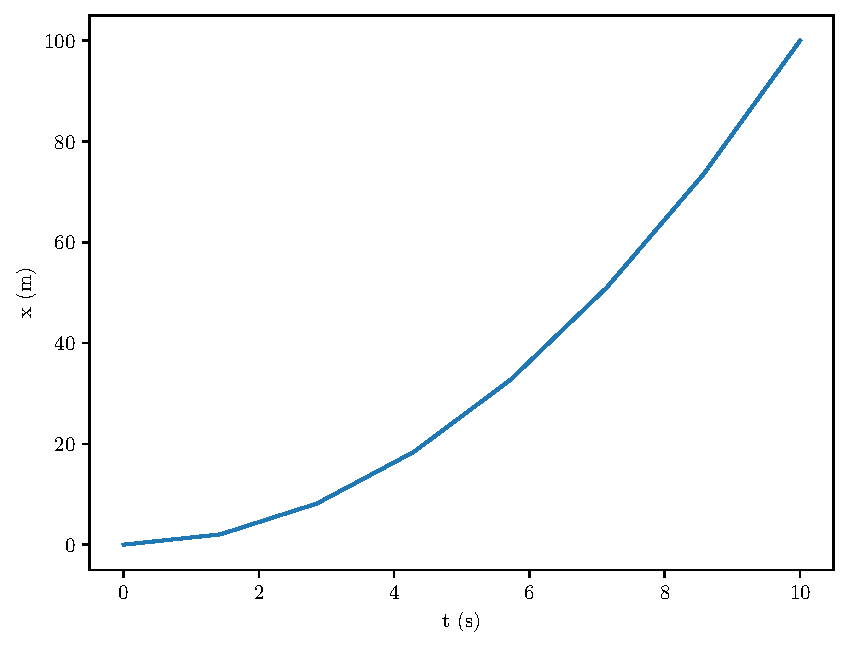
\includegraphics[width=\linewidth]{figures/python_plt-1}
		\captionof{figure}{Figure minimale.}
		\label{fig:mini}
	\end{center}
\end{minipage}
\hfill
\begin{minipage}[t]{.48\linewidth}
	~
	\begin{center}
		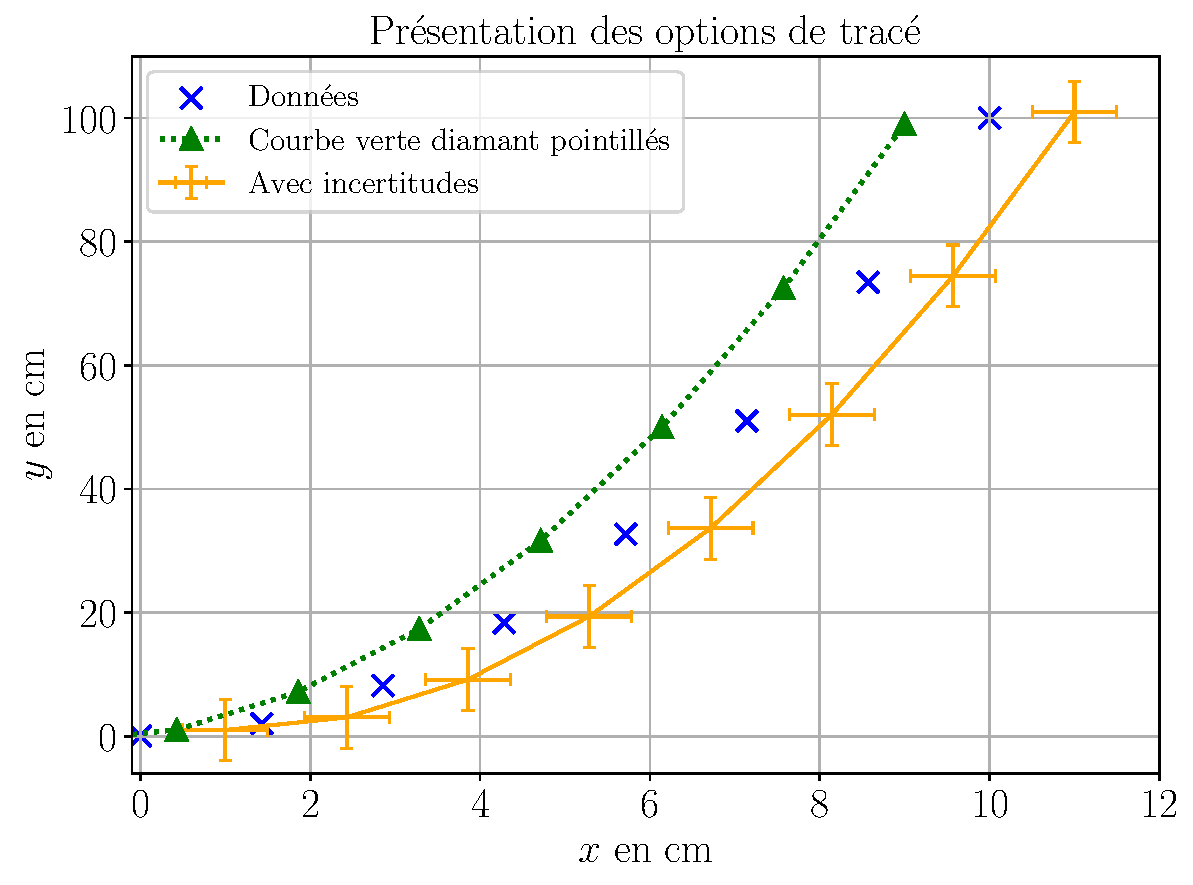
\includegraphics[width=\linewidth]{figures/python_plt-2}
		\captionof{figure}{Figure complexe.}
		\label{fig:cplx}
	\end{center}
\end{minipage}

\subsubsection{Complexe (Figure~\ref{fig:cplx})}
\begin{tcb}[breakable](code)<lfnt>{Code}
	\vspace{-10pt}
	\inputpygments[numbers=left,xleftmargin=10pt]{python}{F05_python_plot-2.py}
\end{tcb}

\section{Simulations \textsc{Monte-Carlo}}
\subsection{Principe}
On dispose généralement de plusieurs jeux de données pour
lesquels on a des incertitudes de mesure, et on veut calculer $z$ qui dépend de
ces données mais d'une manière complexe\ftn{Comprendre~: pas donnée dans la fiche
	\texttt{Mesures et incertitudes}}. On peut alors réaliser une simulation.

En effet, connaissant l'intervalle d'existence des mesures, on peut prendre
aléatoirement d'autres valeurs possibles pour les mesures, et faire toute une
série de calculs avec des valeurs légèrement modifiées. On pourra alors
finalement prendre la moyenne des valeurs calculées et leur écart-type pour
avoir la propagation des incertitudes~!

\begin{tcn}(ror){Cœur de la simulation}
	Finalement, le cœur de la simulation revient (presque) à réaliser une estimation
	d'incertitude de type A sur les valeurs calculées~!
\end{tcn}

\subsection{Application~: mesure d'une distance focale}
On peut mesurer la focale d'une lentille convergente par la méthode de
\textsc{Bessel}~:
\[
	\boxed{f' = \frac{D^{2}-d^{2}}{4D}}
\]
avec $d$ la plage de positions de la lentille qui garde une image nette sur
l'écran, et $D$ la distance objet-écran. S'il est possible de faire le calcul
analytique ici, il peut être plus rapide de réaliser une propagation des
incertitudes des valeurs $d$ et $D$ sur la valeur calculée de $f'$.

Pour cela,
\begin{itemize}
	\item On détermine les demi-largeurs $\Delta_d$ et $\Delta_D$. Si on possède
	      des incertitudes-types, on aura $\Delta_d = u(d)\sqrt{3}$. Sinon, c'est
	      la demi-largeur de la plage des mesures possibles.
	\item On créé une liste \texttt{liste\_f} vide qui accueillera les valeurs de
	      $f'$ calculées~;
	\item On fixe $N \gtrsim \num{e4}$ le nombre de simulations~;
	\item Pour $i$ allant de 0 à $N-1$~:
	      \begin{itemize}
		      \item On tire aléatoirement une valeur de $d$ dans l'intervalle
		            $[d-\Delta_d, d+\Delta_d]$. On appelle cette valeur
		            \texttt{d\_simu}~;
		      \item On tire aléatoirement une valeur de $D$ dans l'intervalle
		            $[D-\Delta_D, D+\Delta_D]$. On appelle cette valeur
		            \texttt{D\_simu}~;
		      \item On calcule $f'$ avec ces données \textbf{simulées}~;
		      \item On ajoute cette valeur simulée à la liste des valeurs de $f'$.
	      \end{itemize}
	\item On a alors $N$ valeurs de $f'$. La valeur la plus probable
	      sera la moyenne, et son incertitude-type est l'écart-type de
	      la liste des $f'$ simulés.
\end{itemize}
\begin{tcn}(defi)<lftt>"info"{Tirage aléatoire}
	\texttt{np.random.uniform(min, max)} est la fonction \texttt{Python} qui permet
	de tirer aléatoirement une valeur entre \texttt{min} et \texttt{max}.
\end{tcn}

Ainsi, en \texttt{Python}~:
\begin{tcb}[breakable](code)<lfnt>{Code}
	\vspace{-10pt}
	\inputpygments[numbers=left,xleftmargin=10pt]{python}{F05_python_mont-1.py}
\end{tcb}

\subsection{Application~: régression linéaire}
Prenons l'exemple de la régression linéaire~:
\[
	y = ax+b
\]
On a mesuré $x$ et $y$, et on obtient $a$ et $b$ avec \texttt{np.polyfit(x, y,
	1)}. Mais ce calcul ne donne pas l'incertitude sur $a$ et $b$. Les deux
valeurs étant interdépendantes, on n'a pas d'expression analytique pour les
déterminer~: on va donc les simuler.

Chaque valeur des $x_i$ est comprise dans un certain intervalle $[x \pm
			\Delta_x]$, et de même pour $y$. Plutôt que de prendre la valeur centrale et de
calculer $a$ et $b$ avec ces valeurs, on peut essayer de calculer $a$ et $b$
pour des valeurs de $x_i$ et de $y_i$ légèrement modifiées, à l'interieur de
l'intervalle des valeurs possibles.

On va donc réaliser un \textbf{grand nombre de régressions linéaires} en
\textbf{prenant des valeurs $x_i$ et $y_i$ «~simulées~»}. On obtient une liste
de valeurs possibles de $a$ et de $b$~; la moyenne des $a$ et $b$ sont alors la
valeur moyenne de la liste, et l'incertitude-type sera l'écart-type de la liste.

\subsection{En pratique}
\begin{itemize}
	\item On détermine les demi-largeurs $\Delta_x$ et $\Delta_y$. Si on possède
	      des incertitudes-types, on aura $\Delta_x = u(x)\sqrt{3}$. Sinon, c'est
	      la demi-largeur de la plage des mesures possibles.
	      \begin{center}
		      \begin{tcn}[cnt](prop)"bomb"{Attention~!!}
			      \Large Pour la régression linéaire, les $\Delta_x$ et $\Delta_y$
			      doivent être des listes~! Il doit y avoir autant de valeurs de
			      $\Delta$ que de valeurs de $x$~!
		      \end{tcn}
	      \end{center}
	\item On fixe un nombre $N$ très grand.
	\item On créé des listes vides \texttt{liste\_a} et \texttt{liste\_b} pour y
	      stocker les futures valeurs des $a$ et des $b$ calculés.
	\item Pour chaque $i$ compris entre $0$ et $N-1$~:
	      \begin{itemize}
		      \item on prend \texttt{x\_simu} dans l'intervalle $[x-\Delta_x,
					            x+\Delta_x]$~;
		      \item on prend \texttt{y\_simu} dans l'intervalle $[y-\Delta_y,
					            y+\Delta_y]$~;
		      \item on calcule \texttt{a\_simu} et \texttt{b\_simu} avec ces valeurs
		            simulées~;
		      \item on les stocke dans \texttt{liste\_a} et \texttt{liste\_b}.
	      \end{itemize}
	\item On a alors $N$ valeurs de $a$ et de $b$~: les valeurs les plus probables
	      sont les moyennes, et leurs incertitudes-types sont les écarts-types des
	      listes de $a$ et de $b$.
\end{itemize}

Ainsi, en \texttt{Python}~:
\begin{tcb}[breakable](code)<lfnt>{Code}
	\vspace{-10pt}
	\inputpygments[numbers=left,xleftmargin=10pt]{python}{F05_python_mont-2.py}
\end{tcb}

\end{document}
